\chapter{Methodology}
    Through this chapter, I will introduce the setting of my work and my data, which in turn leads to the data preparation, and how my experiments were to be conducted. 
    
    \section{The setting} \label{setting}
        The work was conducted over a two-year period from August 2020 to June 2022 at the University of Bergen. My task was provided by the \gls{imr} and so I was invited to regular meetings with their machine learning group as well as the \gls{crimac} group. The initial task developed from an interest in the individual frequency performance of the frequencies involved in the work described in section \ref{unet_paper_acoustic} and I were to base the work I did on their work. Initially, access was granted by the University, to a local server I will call \textit{janus} but later to a new more powerful server called \textit{birget}. These servers were intended to be the locations to run the heavy machine learning algorithms, as these needs to run for long spans of time and had the storage capacity for the data. 
        
        \subsection{The data (.raw \& .work)}
            In this section, I will describe my data, and the tools used to access and process it. The data was provided by the \gls{imr}, and were initially presented to me as \textit{.raw} \cite{raw} with corresponding \textit{.work} files separated into yearly trawl missions from 2011 to 2020. The \textit{.raw} is the uncompressed raw output from the echo sounder. The same format is used by cameras before they are converted to, for example, .jpeg. Because they are uncompressed, they do not lose any data, but unfortunately, this also makes them large. The \textit{.work} files are the annotations of the \textit{.raw} files done by operators using a system called the \Gls{lsss}\cite{lsss}. The data from 2020 alone which spanned three months took 240 GB of storage space and was accessed by downloading it through Windows Azure (described in appendix \ref{Windows Azure}).
    
            In the work performed by \gls{crimac} described in section \ref{unet_paper_acoustic}, a pipeline for classifying the acoustic backscatter was created. It could be run as one module, to directly get the predictions from the .raw data, or the submodules could be accessed and run separately. All modules were accessed through docker (described in appendix \ref{Docker}). I will now describe the modules I used in this thesis:
            
            
            \subsubsection{CRIMAC-pipeline modules} \label{CRIMAC-pipeline}
              \begin{figure}[H]
                \centering
                \includesvg[inkscapelatex=false,width=0.7\textwidth,keepaspectratio]{figures/module_overveiw.svg}
                \caption[Module overview]{Module overview and output flowchart. The colors of modules and  their output will stay the same for later illustrations}
              	\medskip 
                \label{Module_overview_fig}
            \end{figure}

            \begin{description}
              \item[$\bullet$ CRIMAC/Preprocessor:] Preprocesses the \textit{.raw} and \textit{.work} to respectively \textit{.zarr} and \textit{.parquet} files. The output \textit{.zarr} file contained several types of measurements from the trawl missions, like location and temperature. The data I extracted was the \gls{sv} data and was represented as a multidimensional array of size \textit{frequency} x \textit{ping} x \textit{range}. \textit{Range} is eqivialent to \textit{depth}. Frequencies can have different resolutions, and you need the different frequencies to have equal size to create uniform frequency dimensions. The module solves this by performing linear interpolation if lower or averaging if larger, all columns of the other frequencies to have the same size as the columns of a main frequency specified by the user, and in my case the 200kHz. \todo{Skift til 38kHz, hvis ikke dette blir fikset. Og legg til forklaring} The \textit{.parquet} file had issues explained in later in this section. The output \textit{.zarr}, file is illustrated in figure \ref{Module_outputs_illustration_fig}:

              \item[$\bullet$ Pretrained CRIMAC/U-Net:] Using a pretrained U-Net model, it produces pixel-based probabilities of size \textit{class} x \textit{ping} x \textit{depth} where values in each pixel summaries to 1 over all classes. The classes are \textit{sandeel}, \textit{other} and \textit{background}. This is illustrated in figure \ref{Module_outputs_illustration_fig}.  By changing the settings, you have the option to train a new U-Net model with the same scheme set up in the original work described in section \ref{unet_paper_acoustic}.
              
              \item[$\bullet$ CRIMAC/Bottom detection:] Identifies the bottom and generates a pixel-based map stored as \textit{.zarr}. This is a 2D array of size \textit{ping} x \textit{depth}. The output is shown in figure \ref{Module_outputs_illustration_fig}:

            \end{description}
            
        
        \begin{figure}[H]
            \centering
            \includesvg[inkscapelatex=false,width=1\textwidth,keepaspectratio]{figures/output_illustration.svg}
            \caption[Module outputs illustration]{Illustrations of the output from the different modules with enlarged examples from each output. This example is a 500x500 crop. The \textit{200kHz} has been transformed to the decibel scale to make the data observable. The color scale is set to be purple at 0, and yellow at 1. White is missing values.}
          	\medskip 
            \label{Module_outputs_illustration_fig}
        \end{figure}
            
            
    
        \subsection{Restrictions}
            Here I will explain three major restrictions which had a heavy impact on the task and is essential to understand my approach to this task.
            \subsubsection{The .zarr format issue}
                It was decided that my task was to use the \textit{.zarr} format, which was the new standard format that the \gls{imr} were to use to handle acoustic \textit{.raw} data. This proved later to be a problem, as the pipeline \gls{crimac} had developed were yet to be compatible with .zarr formatted input data for training new models. The training of new models, as described later in the experiments section, was crucial for my work. The \gls{imr} could not provide a time for when this feature would be developed, and the problem was discovered close to the end of the third semester out of four total semesters. With the remaining time starting to become an issue, it was decided to exclude the training part of the \gls{crimac} pipeline, and solve the task with a different approach and is described in section \ref{Pseudo label}. Furthermore, the complete pipeline could now not be utilized.
            
             \subsubsection{The .work bitmap issue}\label{bitmap_error}
                Earlier, the \textit{.work} file contain the annotations from the operators and would translate to a bitmap for the labels per class. However, these files were found to be full of errors, different formats for storing the labels, or in some cases missing, and caused the \gls{crimac} preprocessor module to crash or give erroneous outputs in the \textit{.parquet} file. This issue had no certain date to be repaired, and appeared at the same time as the \textit{.zarr} training issue was evaluated, and so was deemed not working when planning my further work. This is also why they are not visualized is the illustrations.

            \subsubsection{Servers at the University of Bergen}
                We began to use the server \textit{janus} already during the first semester of the masters program. Over time, we discovered that this server did not have the capacity to facilitate more than some 3-4 students at once and had regular severe issues. The server saw use of professors from the institute and more than 10 students that I personally knew of. This caused heavy restrictions in the processing power afforded to each user and set unfortunate boundaries on our work. 
                
                In late January of the last semester of the masters program, we gained access to a powerful new server named \textit{birget} and this server could meet the needs of my work. However, this was far too late for major parts of my work, as many already had been implemented with the boundaries set by janus. This heavily affected choices for my method, and in particular the amount of data I could use, as the process of acquiring and processing this data was computationally expensive and had to be conducted on janus as birget lacked the software needed.


    \section{Pseudo labels} \label{Pseudo label}
        My experiments involved utilizing the same U-Net architecture as described in section \ref{unet}, and will be explained in depth in section \ref{Experiments}. This method relies on supervised learning, and so each data sample needs a corresponding label. Due to the .zarr and .work file issues, I did not have access to the same labels that were used in the original work \ref{unet_paper_acoustic}, and thad to come up with an alternate solution. This came to be based on what is called pseudo labels. In meetings with the \gls{imr} we came up with the idea to use the output of the model used in \ref{unet_paper_acoustic} as my labels. The reasoning were that the performance of the trained \gls{crimac} U-Net were assessed to be sufficient for my task. I was then able to create labels for all my data.
        
        This would mean that the labels would consist of predictions produced from the four frequencies used in article \ref{unet_paper_acoustic}, namely; 18kHz, 38kHz, 120kHz and 200kHz. These frequencies were also present in my data. These output of the from the \gls{crimac} U-Net were a segmentation map of probabilities in the range [0,1], and so I applied a threshold of 0.8 to convert the values below to 0 and above to 1. Hence, producing a mask for each class \textit{sandeel}, \textit{other} and \textit{background}, and could be used as labels.
        
        \clearpage
        \begin{figure}[H]
        \centering
        
        \subfloat[Low noise background label.]{
        	\label{subfig:correct}
        	\includesvg[inkscapelatex=false,width=0.9\textwidth,keepaspectratio]{figures/data_sample.svg}}
        	%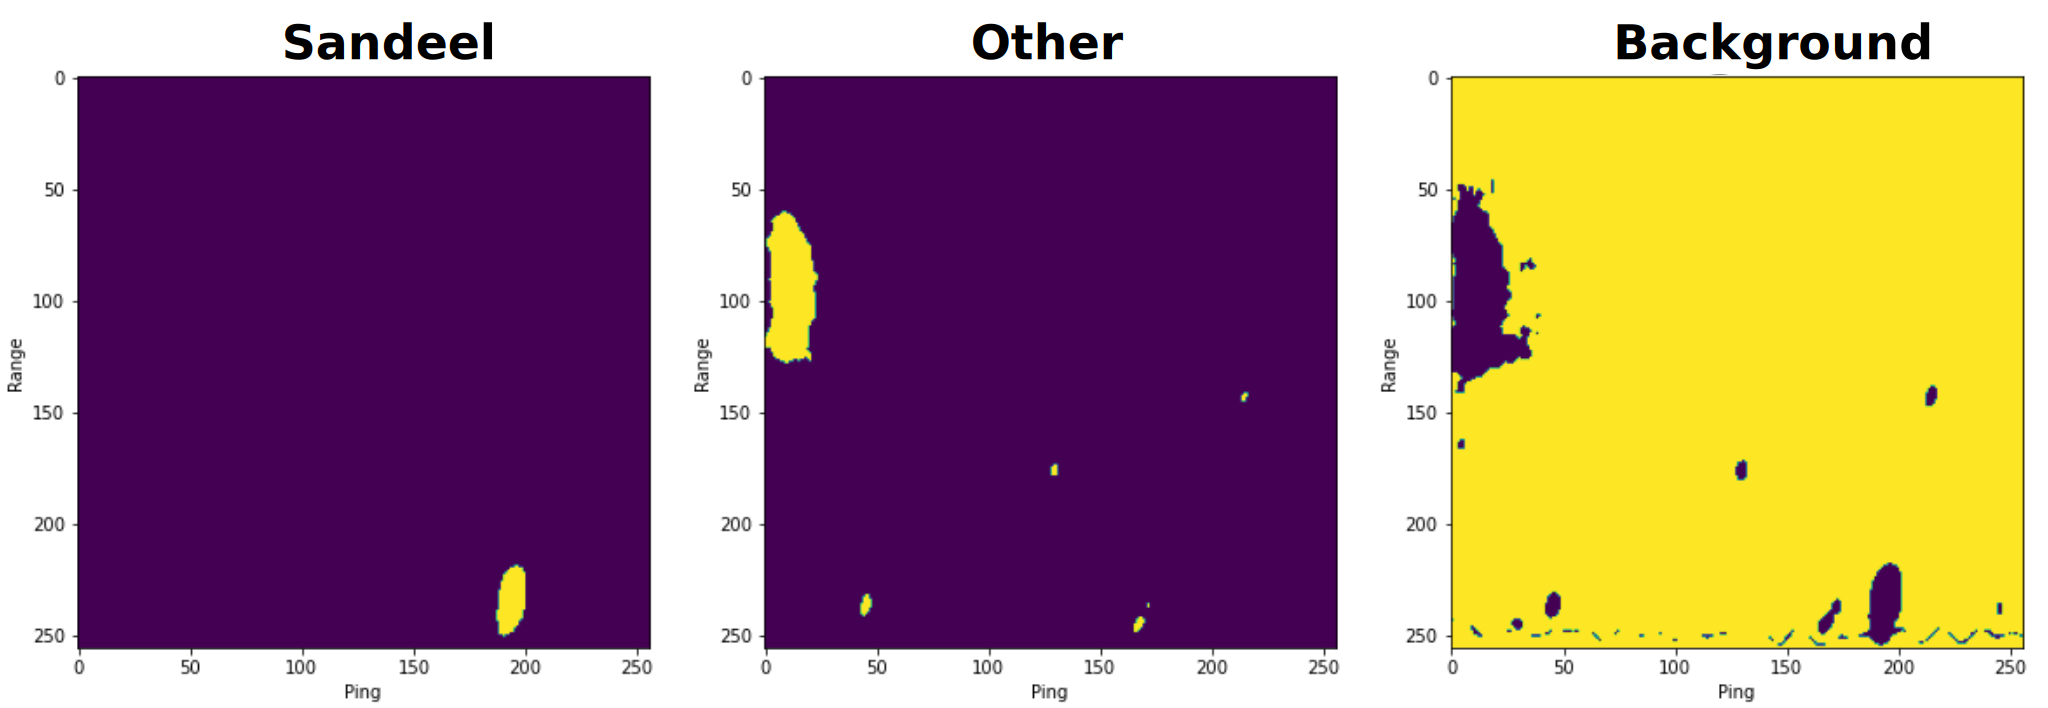
\includegraphics[width=1\textwidth]{figures/data_sample.png} } 
        
        \subfloat[High noise background label.]{
        	\label{subfig:notwhitelight}
        	\includesvg[inkscapelatex=false,width=0.9\textwidth,keepaspectratio]{figures/data_sample_noisy.svg}}
        
        
        \caption[Noise in background comparison]{An example pseudo label displaying the mask of all three classes present in a 256×256 crop. The upper (a) without much noise in the background and the lower (b) containing severe noise.}
        \label{data sample fig}
        
        \end{figure}
        These labels will contain some noise, as the model they originate from was not perfect. In the next section, I will explain how I handled this. Due to the weighted cross-entropy loss used during training of the model seen in section \ref{unet_paper_acoustic} the background class were usually very noisy, as this class was lowly weighted. This low weight caused the model to care less about classifying the background correctly, and the two samples in figure \ref{data sample fig} illustrates this. As I was to use the same weighting, this did not pose a large problem but explains noise in later illustrations of the background class, and therefore mentioned.

        
    \section{Data preparation}
        With the pseudo labels, I possessed all the components I needed to create my own dataset. Here I will go through my implementation of preprocessing the \textit{.raw} data into a dataset able to be quickly loaded into a deep learning algorithm.
        
        \clearpage
        \begin{figure}[H]
            \centering
            \includesvg[inkscapelatex=false,width=0.8\textwidth,keepaspectratio]{figures/flow_data_gen.svg}
            %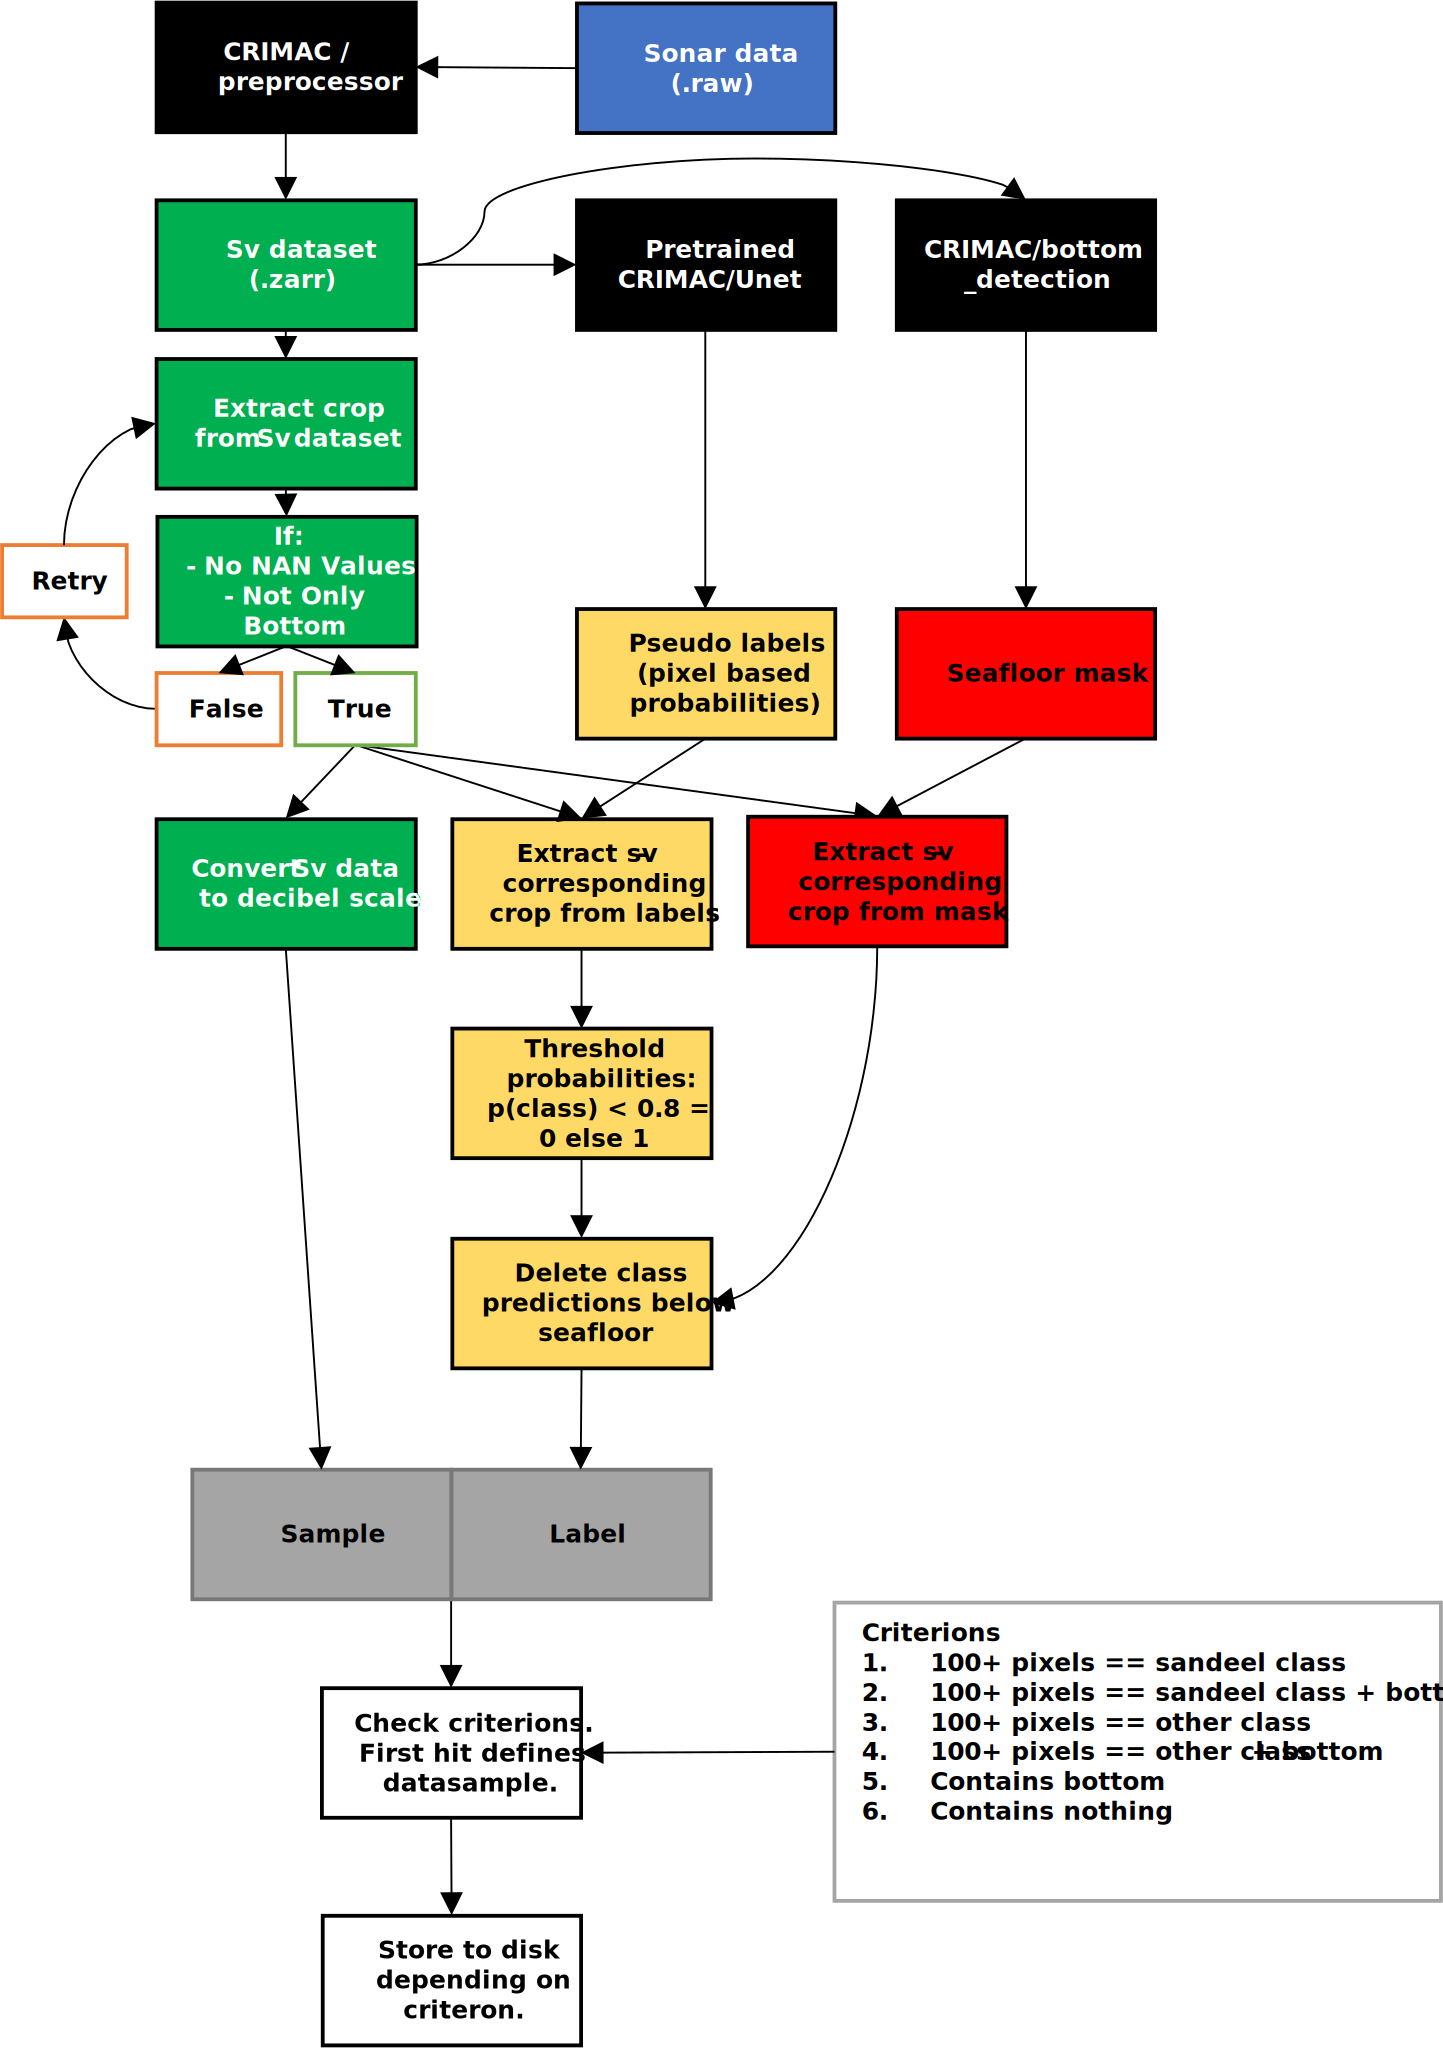
\includegraphics[scale=0.75]{figures/flow_data_gen.png}
            \caption[Data generation process]{An overview of the data generation process. CRIMAC pipeline modules (black), data.raw (blue), SV data.zarr (green), pseudo labels.zarr (yellow), bottom.zarr (red) and the finished file.pytorch (gray).}
          	\medskip 
            \label{data_generation_flowchart_fig}
        \end{figure}
        
        The entire process is illustrated in figure \ref{data_generation_flowchart_fig} and starts with the utilization of \gls{crimac} preprocessor module as described in \ref{CRIMAC-pipeline}. This takes in the entire \textit{.raw} dataset and outputs the \gls{sv} data in the \textit{.zarr} format as a single large array. The \gls{sv} were then sent to both the pretrained U-Net and bottom detection modules from the \gls{crimac} pipeline. The U-Net outputs pseudo labels, and the bottom detection outputs a mask of the seafloor, as arrays equal to the \gls{sv} data array.
        
        \begin{figure}[H]
            \centering
            %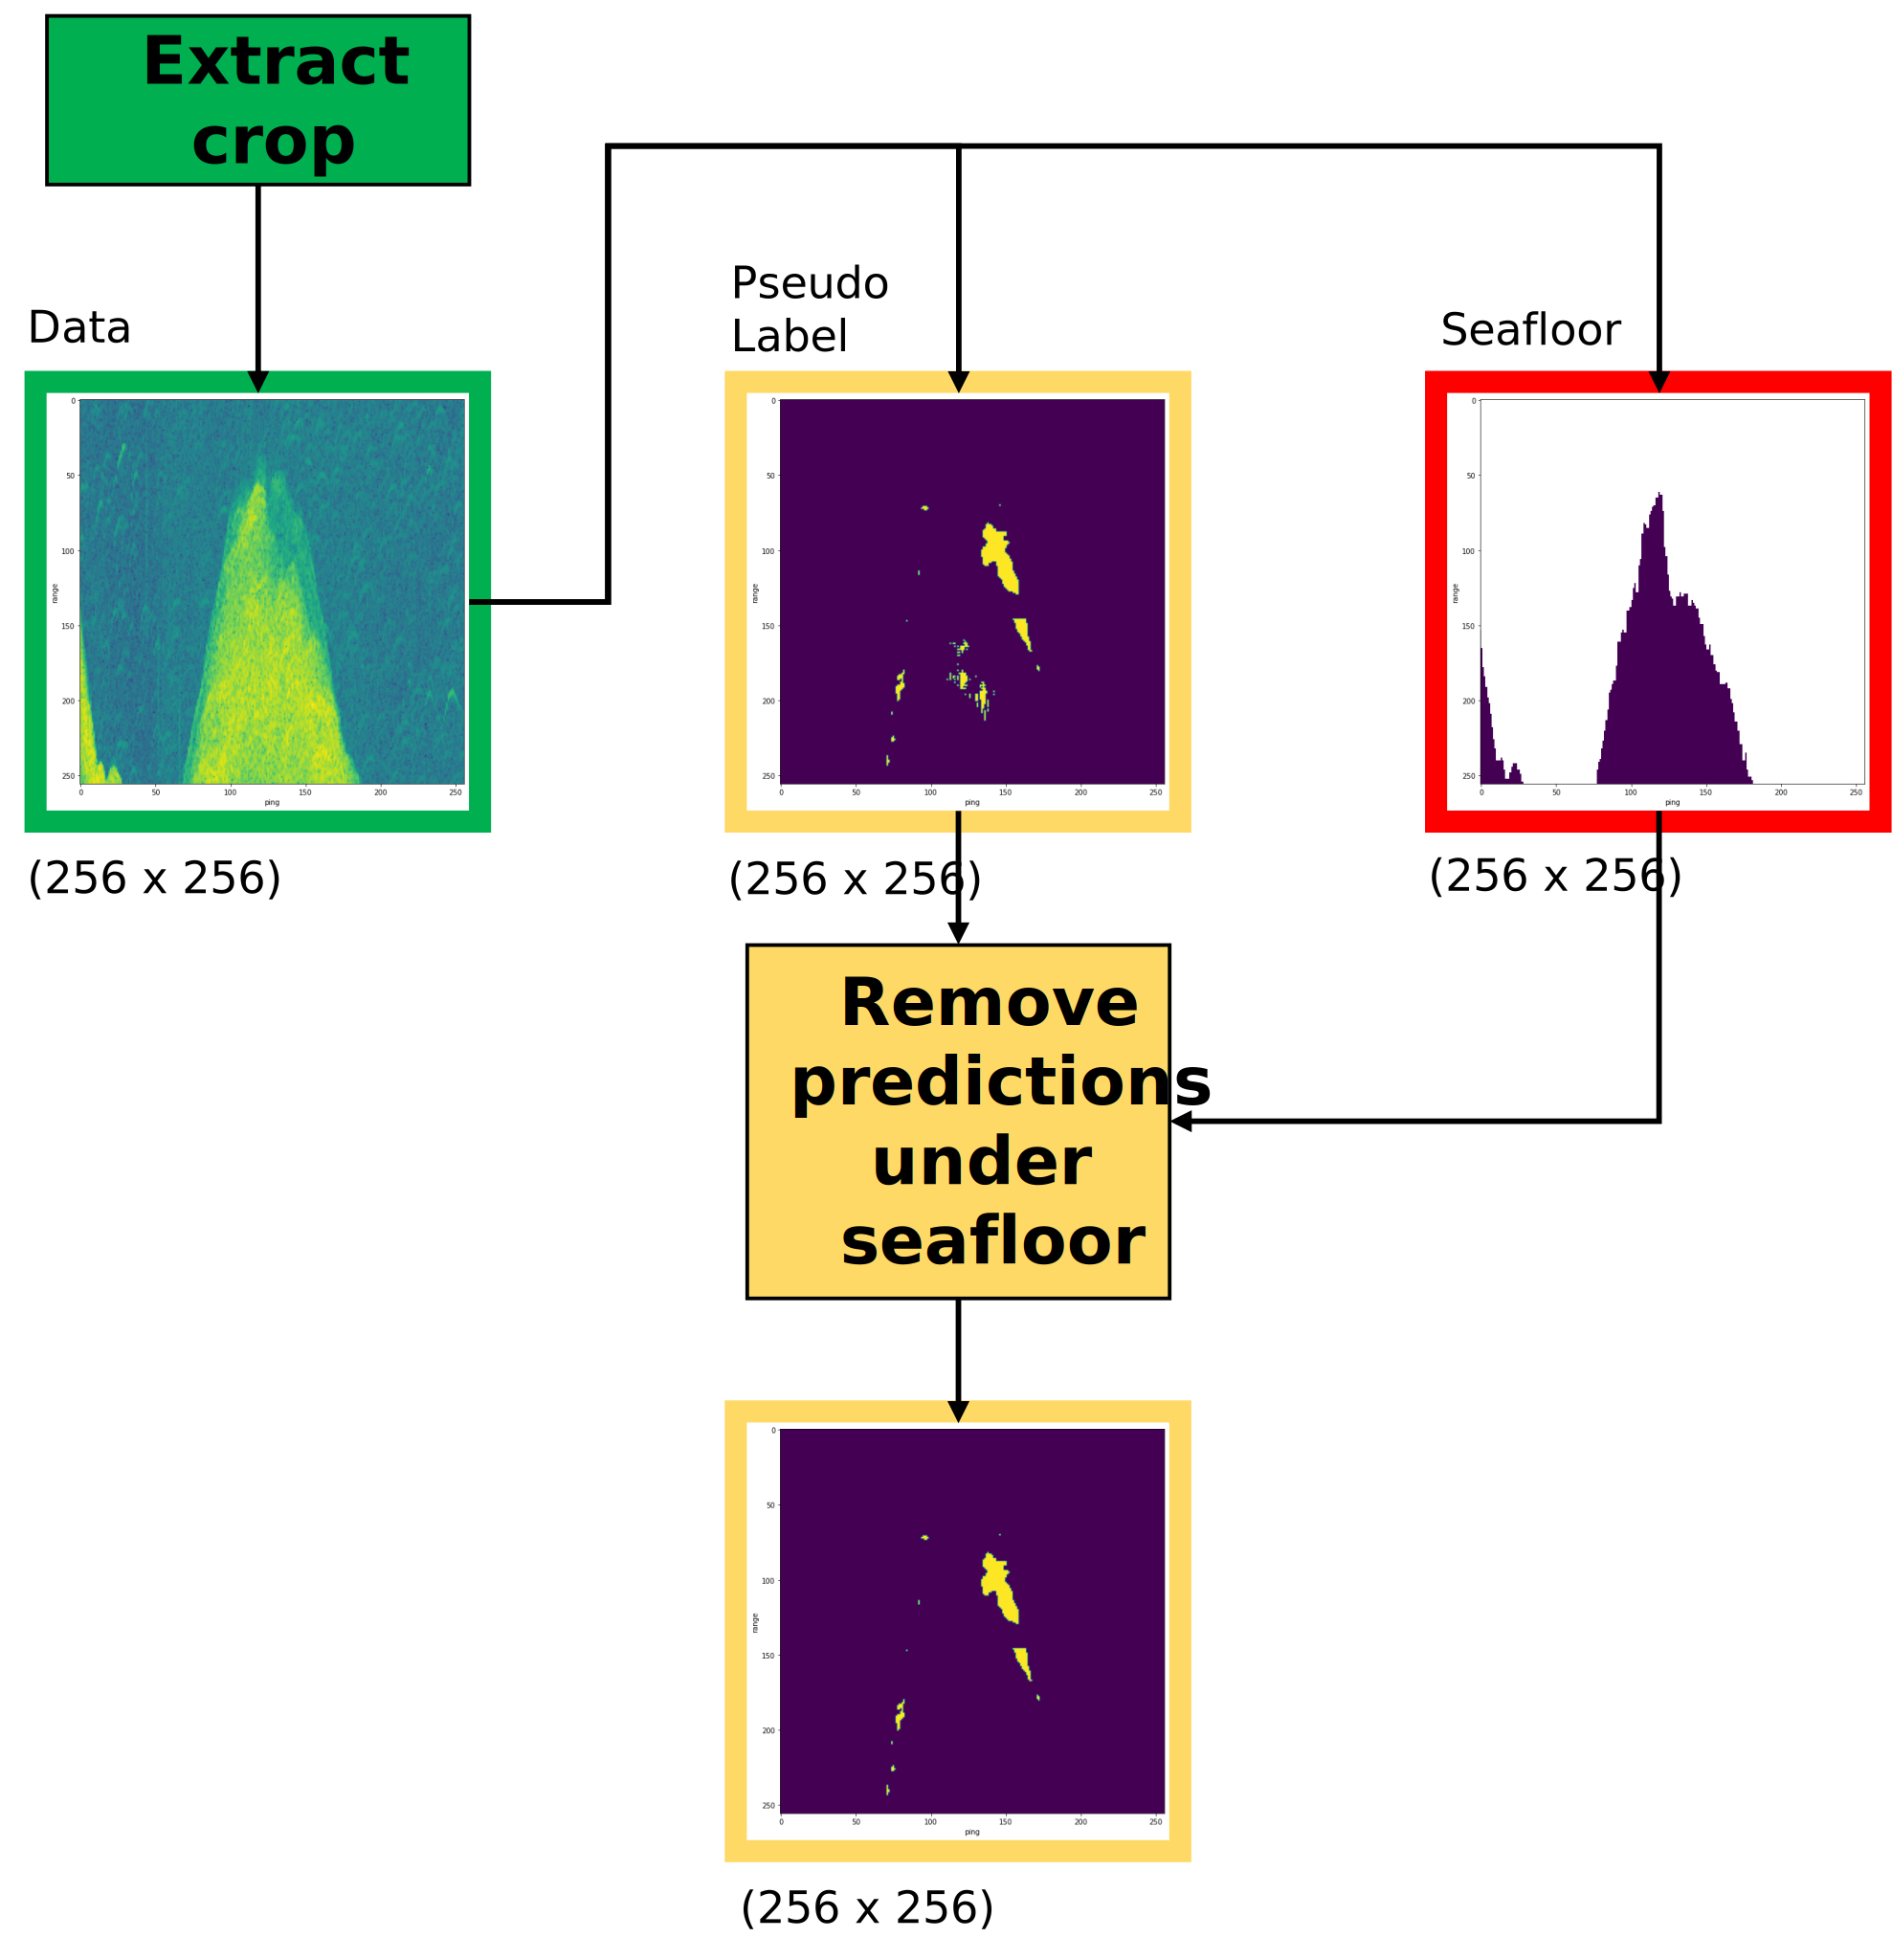
\includegraphics[scale=0.5]{figures/crop_extract_illustration.png}
            \includesvg[inkscapelatex=false,width=0.9\textwidth,keepaspectratio]{figures/data_errors_nans.svg}
            \caption[Missing values and bottom]{Example crop from the 18kHz \gls{sv} data (decibel scale). It illustrates two clear sections of data where the depth (range) is changed, and the gap is filled with missing values (white). The bottom can clearly be observed by the strong line of \gls{sv} values, and there are multiple bottom echoes in certain parts if the crop.}
          	\medskip 
            \label{data_bottom_nans_fig}
        \end{figure}
        
        
        From the \gls{sv} dataset generated, a non-overlapping crop were extracted and was checked for any missing values or the crop being located entirely below the seafloor. This was because missing values can ruin the training process, and crops below the seafloor was excluded in the work done by \gls{crimac} (section \ref{unet_paper_acoustic}). An illustration can be viewed in figure \ref{data_bottom_nans_fig}. The mentioned crop extraction process was repeated until the algorithm found a crop that did not trigger any of the previous two statements. Then, using the vertical and horizontal coordinates from the \gls{sv} data, a corresponding crop from both the seafloor mask and the pseudo labels were extracted, as the array sizes were uniform. The two new crops were then used together to remove predictions that appeared under the seafloor, thus cleaning and preprocessing the pseudo labels. The steps explained in this paragraph are also visualized in figure \ref{crop_extract_fig}. 
        \clearpage
        \begin{figure}[H]
            \centering
            %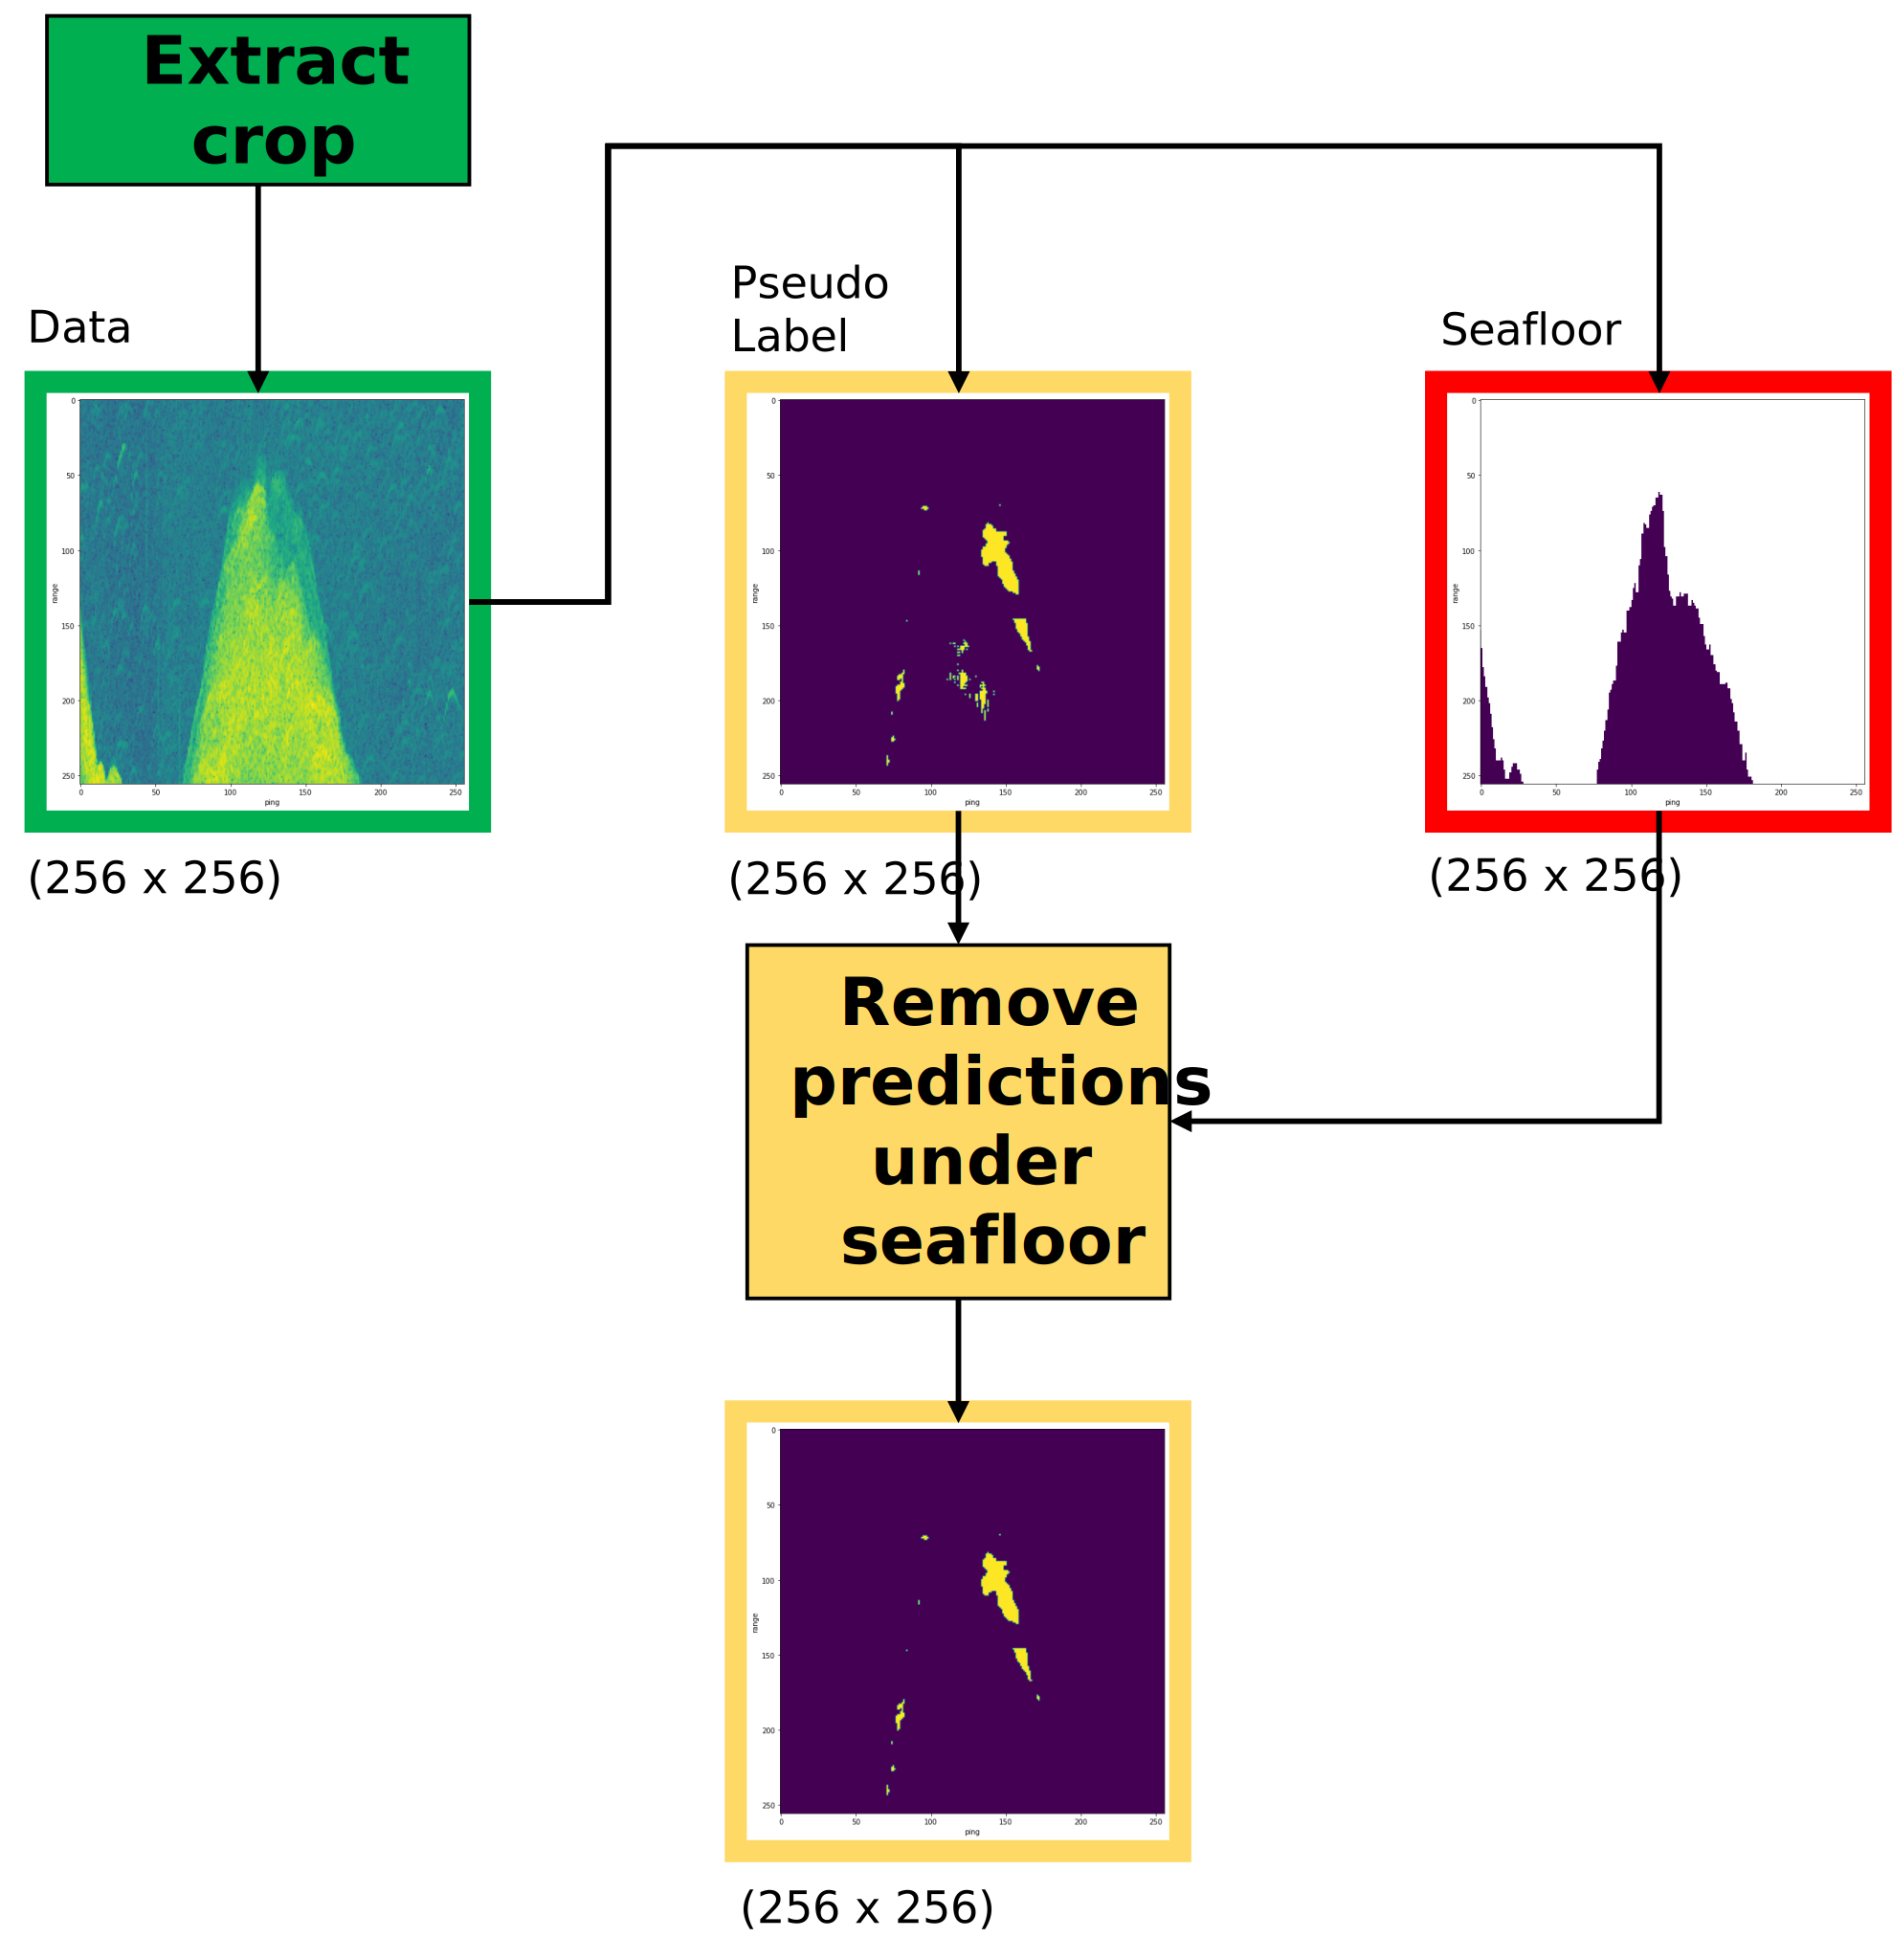
\includegraphics[scale=0.5]{figures/crop_extract_illustration.png}
            \includesvg[inkscapelatex=false,width=0.7\textwidth,keepaspectratio]{figures/crop_extract_illustration.svg}
            \caption[Data, label and bottom crop extraction and interaction]{Example of how the data, pseudo labels and bottom crops would look during data generation. For the pseudo label, purple is values of 0 and yellow value of 1. In the pseudo labels, you can see that some predictions under the seafloor are removed.  Size is shown in the lower-left corner to make it clear that it is a crop of the same size from the same location, but from different arrays.}.
          	\medskip 
            \label{crop_extract_fig}
        \end{figure}
        
        After the crop containing the data and cleaned pseudo labels were generated, I combined them both, now as two tensors, into one file that could be stored to the file system. The file was stored to a folder using PyTorch (\ref{Pytorch}) based on some criterions that will be explained shortly, creating a data hierarchy as shown in figure \ref{data_hierarchy_fig}.
        
        
        %\clearpage
        \begin{figure}[H]
            \centering
            %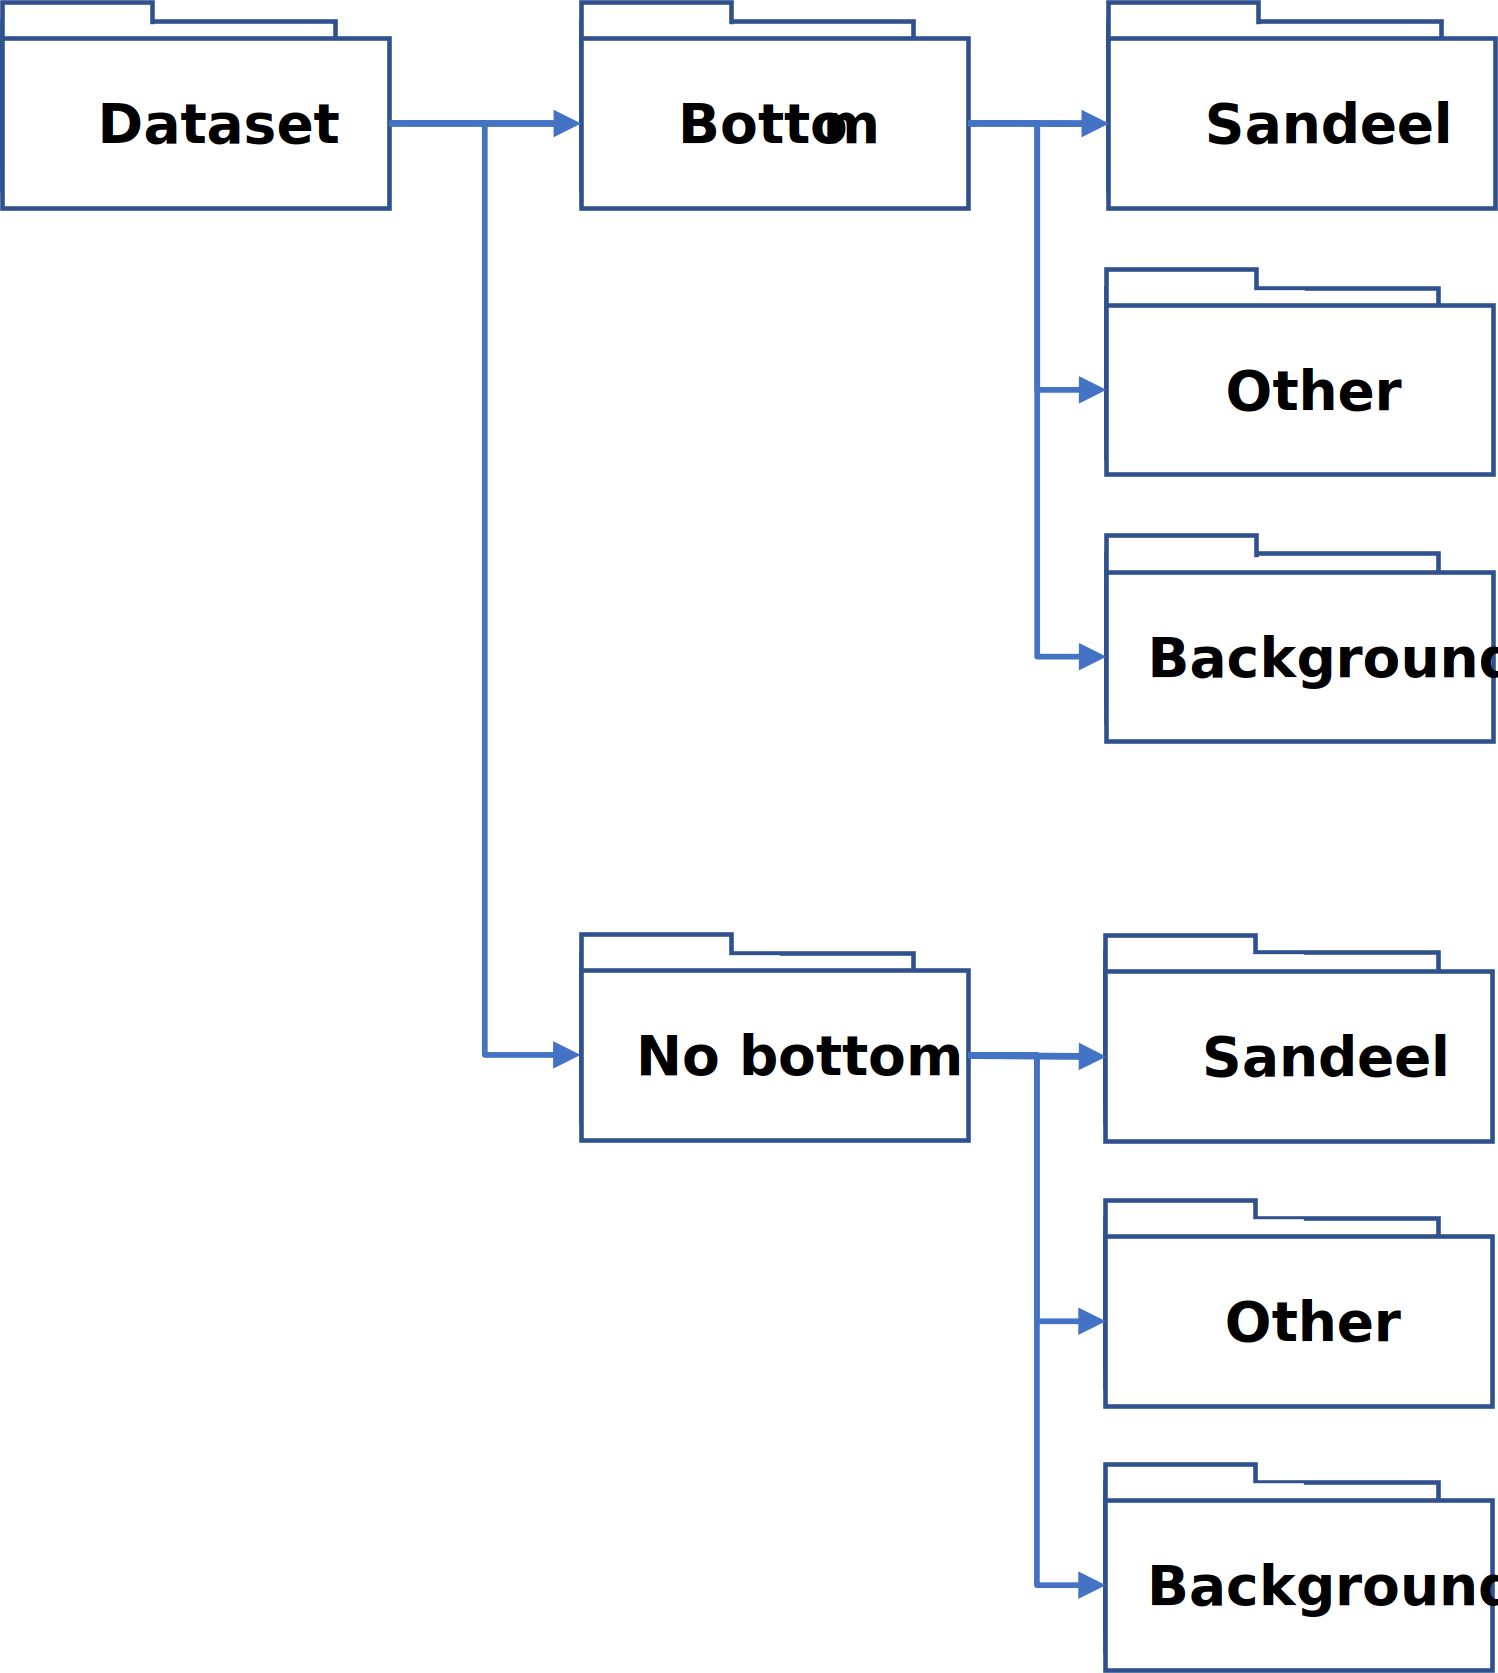
\includegraphics[scale=0.5]{figures/data_hierarki.png}
            \includesvg[inkscapelatex=false,width=0.6\textwidth,keepaspectratio]{figures/data_hierarki.svg}
            \caption[The data-hierarchy]{An overview of the data hierarchy. Two main branches, one with the bottom and one without.}.
          	\medskip 
            \label{data_hierarchy_fig}
        \end{figure}
        
        The criterions were based on those stated in the \ref{unet_paper_acoustic} article and can be seen in figure \ref{data_generation_flowchart_fig} in a box in the lower-right corner. In the previously referenced article, they had the real annotations to know if there was \textit{sandeel} or instances of the \textit{other} class in a crop. I had to rely on the pseudo labels for the same task. Since these labels could be noisey, I set a filter where 100 of the pixels in the crop had to belong to a single class to satisfy my criteria. If there were not enough pixels of either class, the crop would be set to be \textit{valid}. \textit{Valid} can hence forth be thought of as synonymous with \textit{background}. The crop from the bottom was checked to see if any bottom was present, splitting the data into folders with or without bottom. To mitigate duplicate samples, the criteria would be checked from the top to the bottom of the criterion list and store the crop to a folder depending on the first criterion hit.
        
        The loop extracting crops from the \gls{sv} data would continue until the end of the \gls{sv} dataset \textit{.zarr} file.  The process of generating data from a single year took around 1 to 3 days and close to all capacity on the server. Due to these issues, I chose two years as my dataset. In dialogue with the \gls{imr} I chose the year 2018 and 2019 as these were known to have few errors associated with them. The final data distribution can be seen in table \ref{data_distribution_table}.
        
        %\clearpage
        \begin{table}[H]
        \caption[Data distribution]{Data distribution for 2019 and 2018.}.
        \begin{tabular}{|llll|l|l|lllll|l|l}
        \cline{1-5} \cline{7-12}
        \multicolumn{4}{|l|}{\textbf{2018 dataset}}                                             & \% of dataset &  & \multicolumn{5}{l|}{\textbf{2019 dataset}}                                             & \% of dataset &  \\ \cline{1-5} \cline{7-12}
        \multicolumn{2}{|l|}{\multirow{3}{*}{No bottom}} & \multicolumn{1}{l|}{Sandeel} & 1410  & 7.3\%         &  & \multicolumn{3}{l|}{\multirow{3}{*}{No bottom}} & \multicolumn{1}{l|}{Sandeel} & 1308  & 4.38\%        &  \\ \cline{3-5} \cline{10-12}
        \multicolumn{2}{|l|}{}                           & \multicolumn{1}{l|}{Other}   & 184   & 0.95\%        &  & \multicolumn{3}{l|}{}                           & \multicolumn{1}{l|}{Other}   & 1074  & 3.60\%         &  \\ \cline{3-5} \cline{10-12}
        \multicolumn{2}{|l|}{}                           & \multicolumn{1}{l|}{Valid}   & 6519  & 33.75\%       &  & \multicolumn{3}{l|}{}                           & \multicolumn{1}{l|}{Valid}   & 10291 & 34.45\%       &  \\ \cline{1-5} \cline{7-12}
        \multicolumn{2}{|l|}{\multirow{3}{*}{Bottom}}    & \multicolumn{1}{l|}{Sandeel} & 1297  & 6.71\%        &  & \multicolumn{3}{l|}{\multirow{3}{*}{Bottom}}    & \multicolumn{1}{l|}{Sandeel} & 1652  & 5.53\%        &  \\ \cline{3-5} \cline{10-12}
        \multicolumn{2}{|l|}{}                           & \multicolumn{1}{l|}{Other}   & 840   & 4.35\%        &  & \multicolumn{3}{l|}{}                           & \multicolumn{1}{l|}{Other}   & 2815  & 9.42\%        &  \\ \cline{3-5} \cline{10-12}
        \multicolumn{2}{|l|}{}                           & \multicolumn{1}{l|}{Valid}   & 9067  & 46.94\%       &  & \multicolumn{3}{l|}{}                           & \multicolumn{1}{l|}{Valid}   & 12733 & 42.62\%       &  \\ \cline{1-5} \cline{7-12}
        \multicolumn{3}{|l|}{\textbf{Total}}                                            & 19317 & 100\%         &  & \multicolumn{4}{l|}{\textbf{Total}}                                            & 29873 & 100\%         &  \\ \cline{1-5} \cline{7-12}
        \end{tabular}
        \label{data_distribution_table}
        \end{table}
        
        From the table \ref{data_distribution_table} I observed that as in article \ref{unet_paper_acoustic} most of the data will contain no fish, here represented as \textit{valid}.

\clearpage
\section{Experiments} \label{Experiments}
    The experiments revolved around manipulating the number of frequencies given as input to the model and then evaluate performance. In this section, I will describe how my experiments were performed and my thought process around evaluation performance. 
    
    \subsection{Experiment settings} \label{Experiment settings}
        All models are based on the one created in article \ref{unet_paper_acoustic}. In this section, all settings are summarized, and stay the same for all experiments.
        The architecture itself can be seen in figure \ref{unet_fig}, with the only alternation being the number of channels in the input layer. This would range from 1…6 channels, being the number of frequencies included. 
        
        Data loaded to the model started with first selecting a folder from the hierarchy as seen in table \ref{Data_loading_scheme_table},with a set probability for each. Then a sample would be extracted at random from this folder. 
        
        %\clearpage
        \begin{longtable}{lcl}
            \caption[Data loading scheme]{The sample classes correspond to the hierarchy described in figure \ref{data_hierarchy_fig}. Each is given a probability of being the target folder for sample extraction.}
            \\\hline
            \multicolumn{1}{|l|}{\textbf{Sample class}} & \multicolumn{1}{l|}{\textbf{Probability}} & \multicolumn{1}{l|}{\textbf{Details}}                                                         \\ \hline
            \endfirsthead
            %
            \endhead
            
            %
            Sandeel                                     & 5/26                                      & Random crop containing the sandeel class                                                      \\ \hline
            Other                                       & 5/26                                      & Random crop containing the other class                                                        \\ \hline
            Valid                                       & 1/26                                      & Random crop containing no fish                                                                \\ \hline
            Sandeel + bottom                          & 5/26                                      & \begin{tabular}[c]{@{}l@{}}Random crop containing the sandeel class\\ + seafloor\end{tabular} \\ \hline
            Other + bottom                             & 5/26                                      & \begin{tabular}[c]{@{}l@{}}Random crop containing the other class\\ + seafloor\end{tabular}   \\ \hline
            Valid + bottom                        & 5/26                                      & \begin{tabular}[c]{@{}l@{}}Random crop containing no fish\\ + seafloor\end{tabular}           \\ \hline
            \label{Data_loading_scheme_table}
        \end{longtable}

        The augmentations performed was flipping along the vertical axis, and random a multiplicative noise to 5\% of pixels in an input echogram. Then the echogram would always be converted to the decibel scale, with cutoff values at minimum -75db and maximum 0db. Augmentations are summaries in table \ref{data_augmentation_table}.
        
        %\clearpage
        \begin{longtable}{lll}

            \caption[Data augmentation summary]{Description of each data augmentation performed.}
            \\\hline
            \multicolumn{2}{|l|}{\textbf{Data augmentation}} & \multicolumn{1}{l|}{\textbf{Details}} \\ \hline
            \endfirsthead
            %
            \endhead
            %
            \textit{Add noise to 5\% of pixels.}      &       & 50\% of occurring upon loading sample \\ \hline
            \textit{Flip along vertical axis}        &       & 50\% of occurring upon loading sample \\ \hline
            \textit{Convert to decibel scale}        &       & Min -75db, max 0db                    \\ \hline
            \label{data_augmentation_table}
        \end{longtable}
        
        The hyperparameters used during training are summarized in table \ref{hyperparameter_table}.

        \begin{longtable}{lll}
            
            \caption[Experiment hyperparameters]{Settings for all hyperparameters used during the training.}\\
            \\ \hline
            \multicolumn{1}{|l|}{\textbf{Hyperparameters}} & \multicolumn{1}{l|}{\textbf{Value/ Category}} & \multicolumn{1}{l|}{\textbf{Details}}                                                 \\ \hline
            \endfirsthead
            %
            \endhead
            %
            \textit{Loss function:}                         & Weighted Cross-entropy                        & \begin{tabular}[c]{@{}l@{}}Background = 1, \\ Other = 25,\\ Sandeel = 30\end{tabular} \\ \hline
            \textit{Optimizer:}                             & Stochastic gradient descent                   &                                                                                       \\ \hline
            \textit{Learning rate:}                         & 0.01                                          & \begin{tabular}[c]{@{}l@{}}Halved every \\ 1000th batch\end{tabular}                  \\ \hline
            \textit{Momentum:}                              & 0.95                                          &                                                                                       \\ \hline
            \textit{Batch size:}                            & 16                                            &                                                                                       \\ \hline
            \textit{Crop size:}                             & 256×256                                       & \begin{tabular}[c]{@{}l@{}}Include all \\ available channels\end{tabular}             \\ \hline
        \label{hyperparameter_table}
        \end{longtable}




        
        For all experiments, the model architecture was based on the U-Net described in section \ref{unet_paper_acoustic}. The only change to the model was the number of channels in the input layer called “input image” with a value of \textbf{4} in figure \ref{unet_fig}. This would range from 1 to 6 to accommodate the currently tested frequencies.
        
        To evaluate the performance of the models, I utilized the F1 score mentioned in section \ref{f1_score}. I also included the precision and recall, as these are provided greater insight to the model's performance.
        
    %\subsection{Experiment: Training on pseudo labels}
    %  This was a preliminary test to establish that training a model on pseudo labels was possible and would achieve acceptable performance. All frequencies would be included, and this would then produce a baseline performance for the later experiments. 
    
    \subsection{Experiment: Exhaustive frequency search}
        This experiment's goal is to answer the research question:
        \begin{itemize}
            \item \textit{“As a lightweight vessel do not have the structural capacity to carry all the six echo sounders the \gls{imr} usually deploy, which ones should be prioritized when classifying sand eel in acoustic data?”}
        \end{itemize}
    
        To find the most impactful frequencies and try to discover hidden synergies between them, a comprehensive test had to be enacted. This experiment would see all combinations of all frequencies being tested. The experiment would be run 5 times so to take the mean of the results,  reducing variance, and be able to display some statistical data for each. Each would have different random state seeds set to enable different model initialization, but mainly the data and augmentations would not be identical. The random state also accommodates reproducibility. With 6 frequencies in total, the amount of possible combinations for each of the testes would be 63, as the order did not matter and the combination with 0 frequencies was excluded.
        
        I observed that the year 2019 in table \ref{data_distribution_table} contained the most data, and this was to be the one used during training. 70\% was to be training data, and 30\% as validation data. The 2018 dataset was set as the test data. The total amount of data given to a model during training was set to 5,000 batches. With a batch size of 16 this corresponds to 80,000 samples ($5,000 * 16$). This was the same amount as used in the \gls{crimac} U-Net model (section \ref{unet_paper_acoustic})
        
        Logging of metrics would occur at different stages during the training process;
            \begin{itemize}
                \item Every minibatch: Calculate running average training loss.
                \item Every minibatch: Logg the running average for both training and validation loss.
                \item Every 500 minibatch: Run model on 100 batches from the validation data, plot one sample output, its label and record running validation loss on each minibatch. Furthermore, calculate F1-score on both training and validation data for every class.
            \end{itemize}
        To accommodate this logging scheme, I split the training process into 50 epochs, with 100 batches in each. This epoch only related to the logging scheme, and not to the data itself. Hence, each epoch is not the entire dataset, but a part of a sequence of data. This is mentioned to not confuse the reader observing the results.
    
        As the logging and random state was equal for all combinations internal in a test, this would create good comparison illustrations of how each combination performed on the same sample. The metrics loss and F1-score would give an indication towards convergence, over-/under-fitting problems and performance. A sanity check would also be performed by observing a prediction of the sandeel class.
        
        After the training of the current combination, the network would be evaluated on 500 batches from the test data, but without any noise added through augmentation. Finally, the F1-score, precision and recall would be calculated for each class and logged in a \textit{.csv} file. Then the next combination would start the entire process afresh with training.
        
        With the results from the 5 separate experiments, each on all 63 possible combinations, I would then calculate the mean performance values of each frequency combination. This would then be used to show these properties:
        \begin{itemize}

            \item Greedy search among the best frequency combinations per number of frequencies possible. For example; The best from all combinations of three frequencies. One greedy search based on each metric; f1-score, precision, and recall.
            \item To observe how unique the performance was for each combination, a plot to illustrate the statistical properties of each will be presented. This will be shown as an error bar, the top of the bar is the max F1-score achieved, and the bottom is the minimum. I chose this presentation because I judged that too few tests had been run for a proper standard deviation to be calculated.
            \item The performance trend of each frequency. This meant I would, for all frequencies, filter out those sets it was a part of and sort these in increasing order. This would produce a line-plot illustrating what performance scores this frequency contributes to and its overall trend.
        \end{itemize}